\clearpage



\begin{appendix}
\clearpage
\appendix

\hypertarget{data-generation-procedure}{%
\section{\texorpdfstring{Data Generation
Procedure\label{app:generation}}{Data Generation Procedure}}\label{data-generation-procedure}}

\textit{Algorithm 2.1.1: Paremeter Estimation}

Input Parameters: domain \(x\in[0,20]\), range \(y\in[10,100]\),
midpoint \(x_{mid}\).

Output: estimated model parameters \(\hat\alpha, \hat\beta, \hat\theta\)

\begin{enumerate}
\def\labelenumi{\arabic{enumi}.}
\item
  Determine the \(y=-x\) line scaled to fit the assigned domain and
  range.
\item
  Map the values \(x_{mid} - 0.1\) and \(x_{mid} + 0.1\) to the \(y=-x\)
  line for two additional points.
\item
  From the set points \((x_k, y_k)\) for \(k = 1,2,3,4\), obtain the
  coefficients from the linear model \(\ln(y_k) = b_0 +b_1x_k\) to
  obtain starting values -
  \(\alpha_0 = e^{b_0}, \beta_0 = b_1, \theta_0 = 0.5\cdot \min(y)\)
\item
  Using the \texttt{nls()} function from the \texttt{stats} package in
  Rstudio and the starting parameter values -
  \(\alpha_0, \beta_0, \theta_0\) - fit the nonlinear model,
  \(y_k = \alpha\cdot e^{\beta\cdot x_k}+\theta\) to obtain estimated
  parameter values - \(\hat\alpha, \hat\beta, \hat\theta.\)
\end{enumerate}

\noindent\textit{Algorithm 2.1.2: Exponential Simulation}

Input Paremeters: sample size \(N = 50\), estimated parameters
\(\hat\alpha\), \(\hat\beta\), and \(\hat\theta\), \(\sigma\) standard
deviation from the exponential curve.

Output Parameters: \(N\) points, in the form of vectors \(\mathbf{x}\)
and \(\mathbf{y}\).

\begin{enumerate}
\def\labelenumi{\arabic{enumi}.}
\item
  Generate \(\tilde x_j, j = 1,..., N\cdot \frac{3}{4}\) as a sequence
  of evenly spaced points in \([0,20]\). This ensures the full domain of
  \(x\) is used, fulfilling the constraints of spanning the same domain
  and range for each parameter combination.
\item
  Obtain \(\tilde x_i, i = 1,...N\) by sampling \(N = 50\) values from
  the set of \(\tilde x_j\) values. This gaurantees some variability and
  potential clustring in the exponential growth curve disrupting the
  perception due to continuity of points.
\item
  Obtain the final \(x_i\) values by jittering \(\tilde x_i\).
\item
  Calculate \(\tilde\alpha = \frac{\hat\alpha}{e^{\sigma^2/2}}.\) This
  ensures that the range of simulated values for different standard
  devaition parameters has an equal expected value for a given rate of
  change due to the non-constant variance across the domain.
\item
  Generate
  \(y_i = \tilde\alpha\cdot e^{\hat\beta x_i + e_i}+\hat\theta\) where
  \(e_i\sim N(0,\sigma^2).\)
\end{enumerate}

\hypertarget{parameter-selection}{%
\section{\texorpdfstring{Parameter Selection
\label{app:parameters}}{Parameter Selection }}\label{parameter-selection}}

For each level of difficulty, we simulated 1000 data sets of
\((x_{ij}, y_{ij})\) points for \(i = 1,...,50\) and \(j = 1...10\).
Each generated \(x_i\) point from \textit{Algorithm 2.1.2} was
replicated 10 times. Then the lack of fit statistic (LOF) was computed
for each simulated data set by calculating the deviation of the data
from a linear line. Plotting the density curves of the LOF statistics
for each level of difficulty choice allows us to evaluate the ability of
differentiating between the difficulty levels and thus detecting the
target plot. In Figure \ref{fig:lof-density-curves}, we can see the
densities of each of the three difficulty levels. While the LOF
statistic provides us a numerical value for discriminating between the
difficulty levels, we cannot directly relate this to the perceptual
discriminability; it serves primarily as an approximation to ensure that
we are testing parameters at several distinct levels of difficulty.

\begin{figure}

{\centering 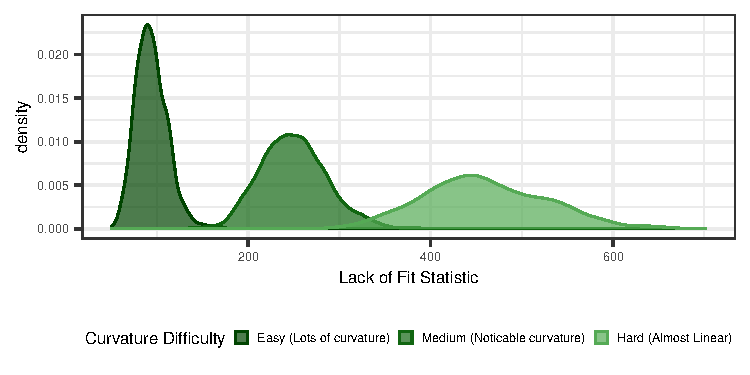
\includegraphics[width=\columnwidth]{./images/lof-density-curves-1} 

}

\caption{Density plot of the lack of fit statistic showing separation of difficulty levels: obvious curvature, noticable curvature, and almost linear.}\label{fig:lof-density-curves}
\end{figure}

Final parameter estimates are shown in Table \ref{tab:parameter-data}.

\begin{table}

\caption{\label{tab:parameter-data}Final parameters used to simulate exponential data for each of the three diffculty levels: Easy (Obvious curvature), Medium (noticable curvature) and Hard (almost linear)}
\centering
\begin{tabular}[t]{ccccccc}
\toprule
 & $x_{mid}$ & $\hat\alpha$ & $\tilde\alpha$ & $\hat\beta$ & $\hat\theta$ & $\hat\sigma$\\
\midrule
Easy & 14.5 & 0.91 & 0.88 & 0.23 & 9.10 & 0.25\\
Medium & 13.0 & 6.86 & 6.82 & 0.13 & 3.14 & 0.12\\
Hard & 11.5 & 37.26 & 37.22 & 0.06 & -27.26 & 0.05\\
\bottomrule
\end{tabular}
\end{table}

\hypertarget{model-details}{%
\section{\texorpdfstring{Model Details
\label{app:glmm-model}}{Model Details }}\label{model-details}}

Target plot identification was analyzed using the Glimmix Procedure in
SAS 9.4. Each lineup plot evaluated was assigned a value based on the
participant response (correct = 1, not correct = 0). Define \(Y_{ijkl}\)
to be the event that participant \(l\) correctly identifies the target
plot for data set \(k\) with curvature \(j\) plotted on scale \(i\). The
binary response was analyzed using generalized linear mixed model
following a binomial distribution with a logit link function following a
row-column blocking design accounting for the variation due to
participant and data set respectively as shown in the Equation (2).
\begin{equation}
\text{logit }P(Y_{ijk}) = \eta + \delta_i + \gamma_j + \delta \gamma_{ij} + s_l + d_k
\end{equation} where

\begin{itemize}
\item $\eta$ is the beaseline average probability of selecting the target plot. 
\item $\delta_i$ is the effect of the log/linear scale.
\item $\gamma_j$ is the effect of the curvature combination.
\item $\delta\gamma_{ij}$is the two-way interaction effect of the scale and curvature.
\item $s_l \sim N(0,\sigma^2_\text{participant})$, random effect for participant characteristics.
\item $d_k \sim N(0,\sigma^2_{\text{data}})$, random effect for data specific characteristics. 
\end{itemize}

We assume that random effects for data set and participant are
independent. See least squares means estimated probabilities in Figure
\ref{fig:lsmeans-plot}.

\begin{figure}

{\centering 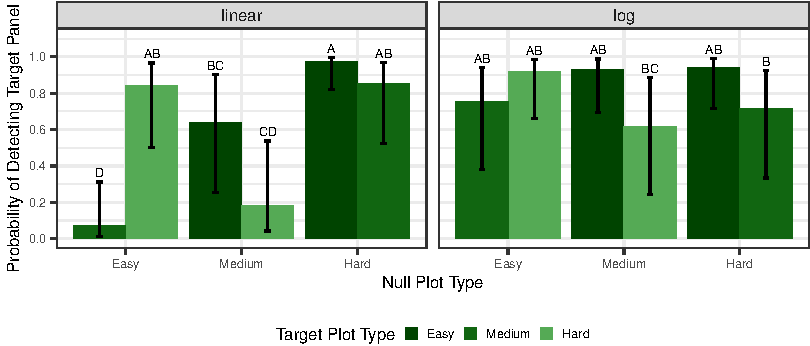
\includegraphics[width=\columnwidth]{./images/lsmeans-plot-1} 

}

\caption{Least Squares Means}\label{fig:lsmeans-plot}
\end{figure}

Type III tests for fixed effects shown in Table
\ref{tab:type3-fixed-effects} indicate a significant interaction between
the curvature combination and scale. Variance due to participant and
data set were estimated to be \(\sigma^2_{participant} = 2.13\) (s.e.
0.74) and \(\sigma^2_{data set} = 0.92\) (s.e. 0.70).

\begin{table}

\caption{\label{tab:type3-fixed-effects}Type III Tests for Fixed Effects}
\centering
\begin{tabular}[t]{cccc}
\toprule
Fixed Effect & F & DF & P-value\\
\midrule
Curvature & 3.66 & 5 , 419 & 0.003\\
Scale & 14.89 & 1 , 419 & 0.0001\\
Curvature x Scale & 6.58 & 5 , 419 & <0.0001\\
\bottomrule
\end{tabular}
\end{table}
\end{appendix}
